% Document class and two-column conversion
\documentclass[twocolumn]{report}
% dimensions of paper and relative text positioning
\usepackage[a4paper,top=2cm,bottom=2cm,left=2cm,right=2cm]{geometry}
% package for including URLs
\usepackage{url}

% Start of the document
\begin{document}

% Title page
\title{\Huge \bfseries A pure Julia implementation of the SG-t-SNE-Pi algorithm} %\Huge and \bfseries are used to make the title bigger and bold
\author{Konstantinos Fotios Papadakis\vspace{0.5cm} \\  AEM:10371} % \vspace{0.5cm} is used to add some vertical space between the author and the AEM
\date{\today}
% prints the title, author and date on a separate page
\maketitle

% Table of contents page
\tableofcontents

% Abstract page
\begin{abstract}
    The Abstract goes here.
\end{abstract}

% Theoretical background chapter
\chapter{Theoretical background}
\section{Introduction to t-SNE}
T-SNE stands for t distributed stochastic neighbor embedding. "T" comes from the type of distribution we use,
Student t-distribution, "Stochastic" comes from the fact that the algorithm is probabilistic in nature, "Neighbor"
comes from the fact that we try to preserve the neighbor relations between data points and finally "embedding"
comes from the fact that we cramp up these relations, in a lower than the initial, dimensional space. t-SNE
is one state-of-the-art technique for dimensional reduction mainly used for visualization purposes. It is a 
way to represent data that reside in a high dimensional space by using a low dimensional graph, all while 
retaining the information of the high dimensional space. To achieve this we have to determine the probability
of two data points being neighbors which can be described by the following equation:
$$P_{i|j} = \frac{exp(-||x_i - x_j||^2 / 2\sigma_i^2)}{\sum_{k \neq i} exp(-||x_i - x_k||^2 / 2\sigma_i^2)}$$

Despite its complicated appearance, it is just a division between two Gaussian probability density functions.
Now, when picking two points at random the probability is given by the following formula that shows how similar
the higher embeddings are:
$$P_{ij} = \frac{P_{i|j} + P_{j|i}}{N}$$

Similarly, the lower embeddings are: 
$$Q_{ij} = \frac{(1 + ||y_i - y_j||^2)^{-1}}{\sum_{k \neq l} (1 + ||y_k - y_l||^2)^{-1}}$$

Because we are moving from a high to a low dimensional space we have limited space to translate the existing
data. This is why there is a need to fit more points in a dimension that wasn't initially designed to fit them.
To solve this problem we use a one-degree-of-freedom Students t-distribution, also known as the Cauchy 
distribution, which has a heavier tail.

To tidy up the previous notions comes the KL divergence, which is a measure of how different two probability
distributions are from each other:
$$KL(P||Q) = \sum_{i \neq j} P_{i|j} log\left(\frac{P_i|j}{Q_i|j}\right)$$

When this nears zero, or ideally becomes zero, we can say that we have successfully migrated from the 
high-dimensional graph to a lower one. Finally, the method we use to minimize the KL divergence is by
applying gradient descent. We consider KL to be a loss function and, after taking its derivative, we
try to minimize it by making slight changes to the $$y_i$$ and $$y_j$$ until the KL divergence is minimized.
\section{Extension of t-SNE to SG-t-SNE (SG-t-SNE-Pi.jl)}
SG-t-SNE-Pi is an extension of t-SNE. It stands for Stochastic Graph t distributed Stochastic Neighbor 
Embedding Pi:
\begin{itemize} 
    \item "Stochastic Graph" means that t-SNE is modified so that it can embed large sparse stochastic 
    graphs into low-dimensional spaces.
    \item "t-SNE" remains as explained in the previous segment of the report. 
    \item "Pi" is used to give name to two new features unique to this version of the algorithm.
    \begin{enumerate}
        \item The accelerated gradient calculation of t-SNE
        \item The faster than cutting edge 2D embedding algorithms, such as FIt-SNE or t-SNE-BH, 3D 
        embedding of t-SNE-Pi  
    \end{enumerate}
\end{itemize}
\cite{SG-tSNE-Pi}
% To-do: use the same source to note the changes that enable these new features

% Benchmarking current implementation chapter
\chapter{Project sgtsnepi_purejulia}
\section{Project's goal}
This project aims to port the C/C++ implementation of SG-tSNE-Pi in the Julia programming language hoping 
to achieve even faster performance. The port has already been partially successful. The code seems to be 
functional but lacks in speed. Thus, in the next segments we will have to go through various utilities to 
map the program's functions and hopefully modify it to get closer to the original implementation's performance.

In order to optimize the code we need to figure out which parts of the code are the most time consuming.
To do this we will use the VsCode profiler which will give us a detailed report consisting of code loops
and their respective time consumption. The parts that take the most time are the ones that we can benefit 
more from optimizing them.

Lastly we will benchmark the code so that we can have a staring point to compare the optimized code with.

\section{Code profiling}
With the help of the VsCode's built in profiler we can form a rough idea of what parts of the code
are taking the longest. Here is the output:
\begin{figure}[H]
    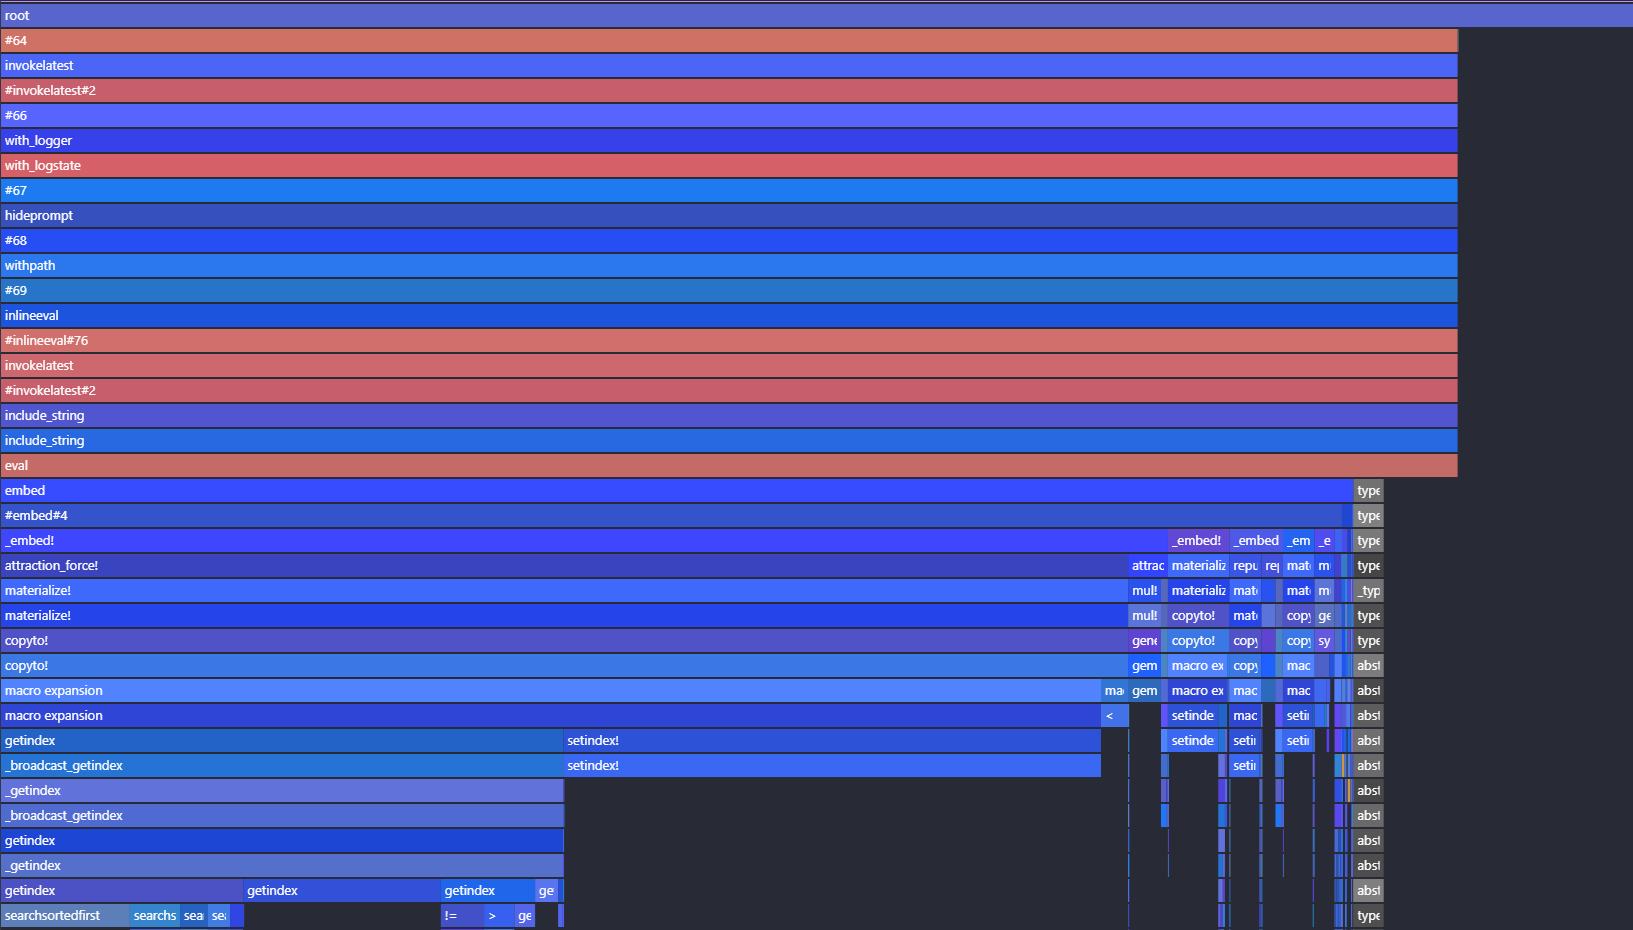
\includegraphics[width=0.5\textwidth]{media/embedProfiling.png}
    \caption{Profiling with attraction\_force!}
\end{figure}
with a profiling time of 132 seconds. \\

After taking a closer look we notice the following resource intensive parts:
\begin{itemize}
    % inclusive time: time spent in the function and all functions it calls
    % exclusive time: time spent in the function itself
    \item function embed, exclusive|20\% or inclusive|83\% 
    \item In embed: z = \_embed!(), exclusive|19\% or inclusive|82\% 
    \item In \_embed!(): attraction\_force!(), exclusive|15\% or inclusive|72\%
    \item In attraction\_force!(): 
    \begin{minted}[breaklines,escapeinside=||,
                mathescape=true, 
                linenos, 
                numbersep=3pt, 
                gobble=2, 
                frame=lines, 
                fontsize=\small, 
                framesep=2mm]{julia}
        PQ .= P .* Q; # exclusive|15% or inclusive|69%
    \end{minted}
\end{itemize}

Since we are using a sparse matrix P we can substitute attraction\_force!() with attraction\_force\_symm!().
This is the main change we will be making to the existing embed function to improve its performance. This
version works for symmetric P matrices, and allows multiple threads to be used. Here we can see the 
new results:
\begin{figure}[H]
    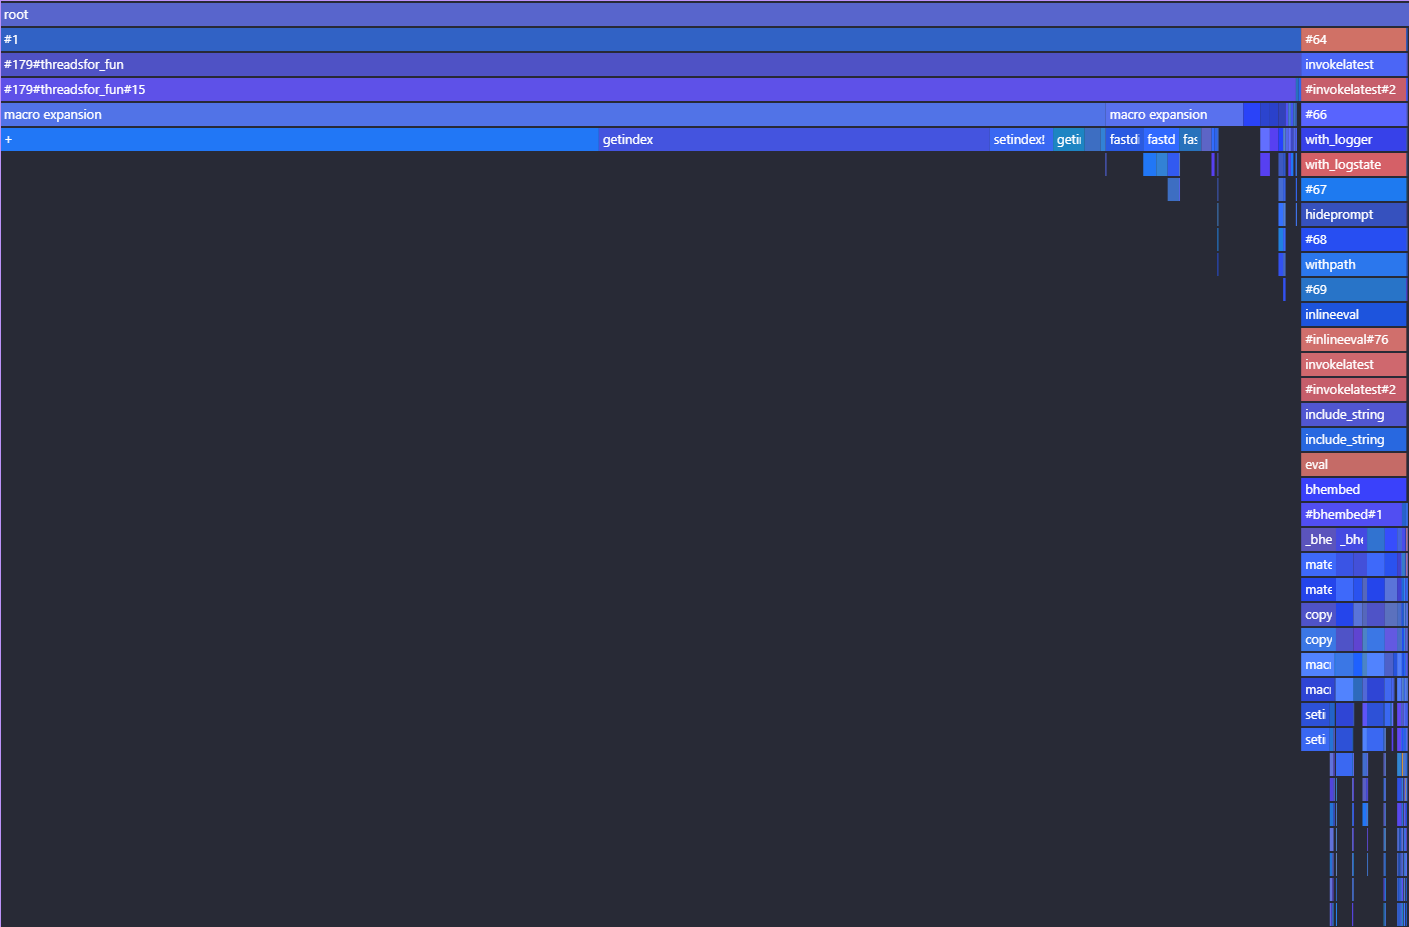
\includegraphics[width=0.5\textwidth]{media/embedProfilingSymm.png}
    \caption{Profiling with attraction\_force\_symm!}
\end{figure}
with a profiling time of 201 seconds. \\

Here the resource intensive parts are:
\begin{itemize}
    \item In attraction\_force!(): 
\end{itemize}
\begin{minted}[breaklines,escapeinside=||,
            mathescape=true, 
            linenos, 
            numbersep=3pt, 
            gobble=2, 
            frame=lines, 
            fontsize=\small, 
            framesep=2mm]{julia}
    Fattr[j,l] += pq * (Yj[l] - Yi[l]) # 78%
\end{minted}

This change introduced a longer profiling time but limited the dependency of the function's speed
to one function which allows us to tweak that one part of the code to improve the overall performance.
It is important to note here that we have not yet set the number of threads for the second version
so the immediately negative results are not indicative of the method's performance. We will later
see exactly how the parameter JULIA\_NUM\_THREADS affects the performance of the function.

% To do: Implement Barnes Hut Algorithm 
% Note that we will be using the "Sparse (without allocations) Barnes-Hut Embeddings" Algorithm.
\section{Benchmarking}
Here we will be testing the following versions of the SG-t-SNE-Pi algorithm:
\begin{itemize}
    \item The original C/C++ implementation of the SG-t-SNE-Pi algorithm.
    \item The pure Julia implementation of the SG-t-SNE-Pi algorithm before the modifications.
\end{itemize}
All the tests where performed on the same machine with the following specifications:
\begin{itemize}
    \item CPU: Intel Core i5-4460 @ 3.20GHz
    \item RAM: 16GB DDR3 787MHz
    \item OS: WSL 2 on Windows 10 Pro 64-bit
    \item Julia version: 1.10.0
\end{itemize}
The P matrix used for our results was set in a pseudo-random manner to ensure reproducibility. The parameters
used can be summed up in the following Julia code:
\begin{minted}[breaklines,escapeinside=||,
                mathescape=true, 
                linenos, 
                numbersep=3pt, 
                gobble=2, 
                frame=lines, 
                fontsize=\small, 
                framesep=2mm]{julia} 
    n = 1000;   # number of points
    d = 10;     # average degree
    
    # Set the random seed for reproducibility
    Random.seed!(42)
    
    # Generate the sparse matrix with a deterministic random pattern
    P = sprand(n, n, d/n)

    # Benchmark the sgtsnepi function
    results=[]
    for i in 1:20
        t=@elapsed SGtSNEpi.embed( P )
        push!(results,t)
    end
\end{minted}
The results of the benchmarks are shown in the following graphs:
\begin{figure}[H]
    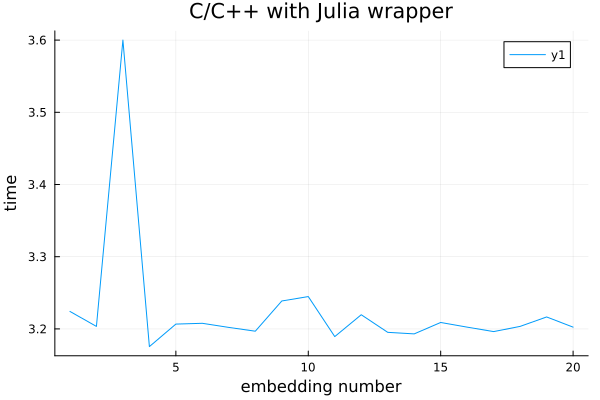
\includegraphics[width=0.5\textwidth]{media/c-c++plot.png}
    \caption{C/C++ with Julia wrapper}
\end{figure}
\begin{figure}[H]
    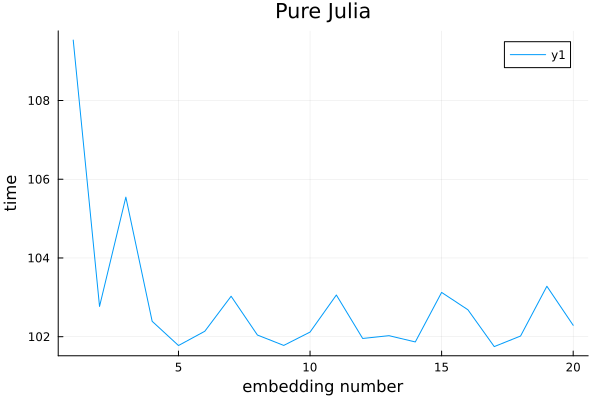
\includegraphics[width=0.5\textwidth]{media/embed.png}
    \caption{Pure Julia}
\end{figure}
\section{Results}
\input{sections/results}

% Times improvement and code modifications chapter
\chapter{Code modifications and time improvements}
\section{Code modifications}
We will now proceed to test the embed function which uses attraction\_force\_symm!() with different 
number of threads to see how the performance is affected. This version of the SG-t-SNE-Pi algorithm is:
\begin{itemize}
    \item The pure Julia implementation of the SG-t-SNE-Pi algorithm after the modifications.
\end{itemize}

To implement this change we create a new julia file called bhembed.jl (Barnes Hut embed) which will
be the same as embed.jl with the only difference being that this one will use the parallelized method of 
calculating the attraction forces.

\section{Time improvements}
Now, to test our efforts we will be going through a detailed comparison between:
\begin{itemize}
    \item The original C/C++ implementation of the SG-t-SNE-Pi algorithm.
    \item The pure Julia implementation of the SG-t-SNE-Pi algorithm before the modifications.
    \item The pure Julia implementation of the SG-t-SNE-Pi algorithm after the modifications.
\end{itemize}
All the tests where performed on the same machine with the following specifications:
\begin{itemize}
    \item CPU: Intel Core i5-4460 @ 3.20GHz
    \item RAM: 16GB DDR3 787MHz
    \item OS: WSL 2 on Windows 10 Pro 64-bit
    \item Julia version: 1.6.1
\end{itemize}
The P matrix used for our results was set in a pseudo-random manner to ensure reproducibility:
\begin{lstlisting}[style=julia]
    using SGtSNEpi, BenchmarkTools, SparseArrays, Random
    
    n = 2000;   # number of points
    d = 10;     # average degree
    
    # Set the random seed for reproducibility
    Random.seed!(42)
    
    # Generate the sparse matrix with a deterministic random pattern
    P = sprand(n, n, d/n)
    my_Y = rand( n, 3 )

    # Benchmark the sgtsnepi function
    results=[]
    for i in 1:20
        t=@elapsed SGtSNEpi.bhembed( P )
        push!(results,t)
    end
\end{lstlisting}
The results of the benchmarks are shown in the following graphs:
\begin{itemize}
    \item C/C++

    \item Julia 

    \item Julia (modified)

\end{itemize}


% Conclusion chapter
\chapter{Conclusions}
\section{Verdict}
Compared to the initial version of the SG-t-SNE-Pi algorithm in c/c++, the pure julia version of the algorithm 
is lacking. After around 8 threads we encounter diminishing returns. We reached a point where we exceeded 
the physical threads enough to gain minimal to no boost in performance. If we had more physical threads 
we could benefit from assigning more Julia threads to the program. However since we want it to be able to 
run on various hardware and the Julia wrapper highlighted significantly better performance on the same 
hardware, the parallelization of the attraction\_force function would have to change. The following profiling 
proves that attraction\_force is still the most costly process:
\begin{figure}[H]
    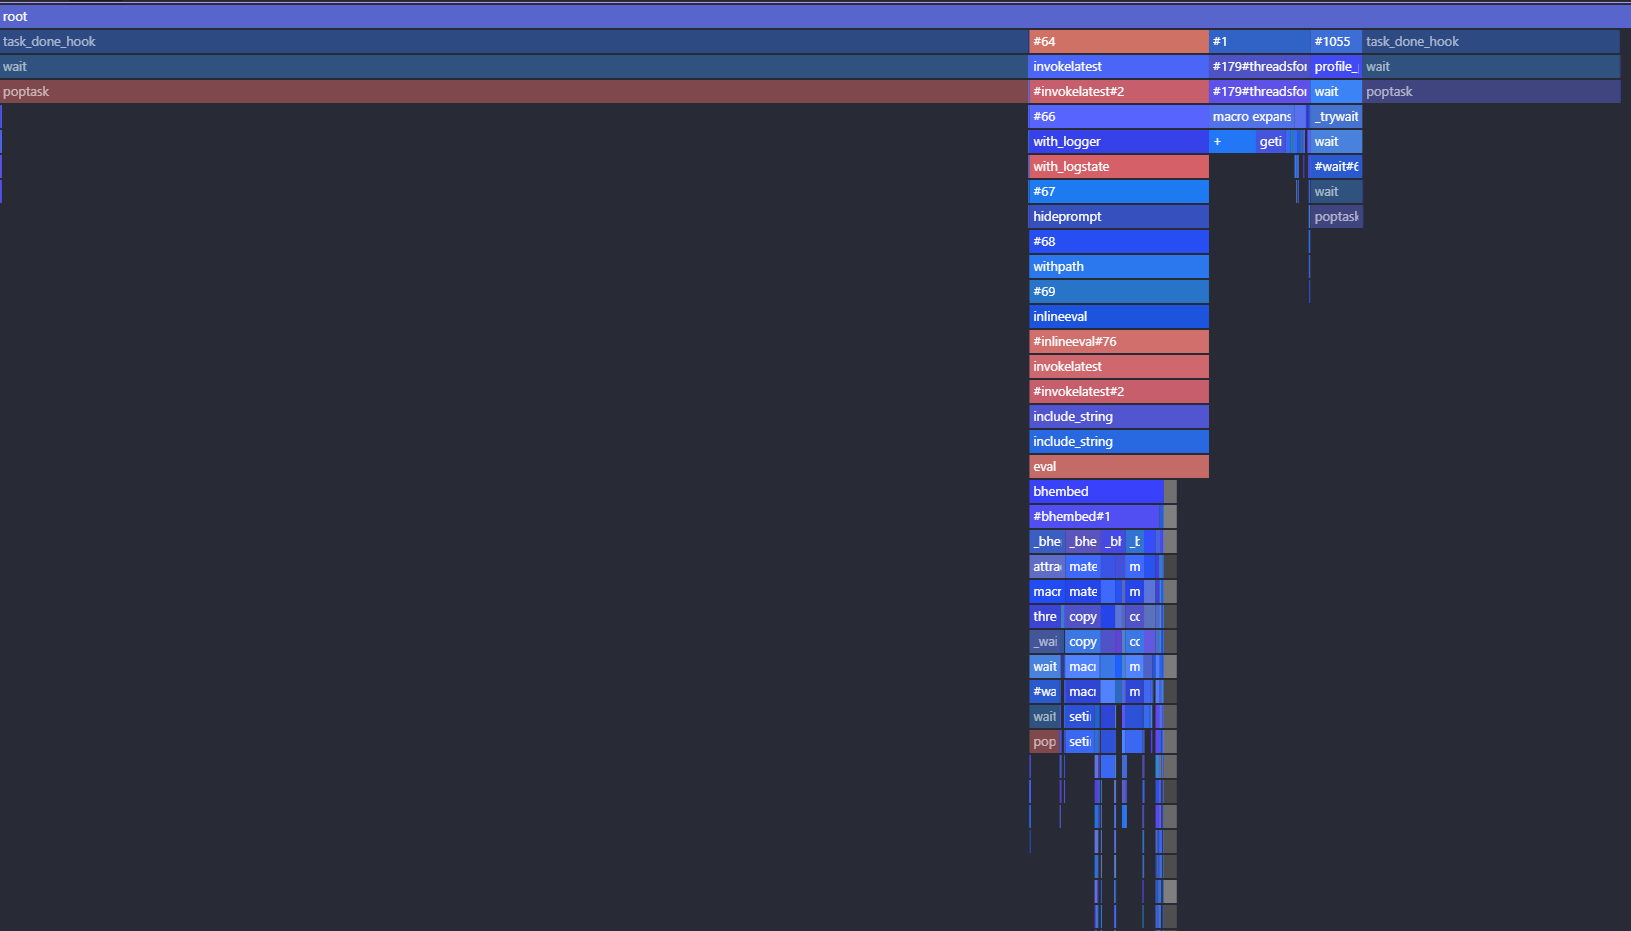
\includegraphics[width=0.5\textwidth]{media/bhembedProfiling.png}
    \caption{Profiling the best pure Julia version}
\end{figure}

To conclude, it seems that the key to advancing the sgtsnepi pure julia project most likely lies in 
finding a better way of parallelizing attraction\_force.


% Bibliography
\nocite{*} % Include all references in the bibliography, even if they are not cited in the report
\bibliographystyle{plain}
\renewcommand{\bibname}{Bibliography}
\bibliography{references/references} % We have to include the references somewhere in the report for them to show here if we don't use (\nocite{*})
\addcontentsline{toc}{chapter}{\bibname}

% End of the document
\end{document}
